The processing layer takes in analog data, digitizes it, and then processes it.  This processed data is then sent to the controller layer.

\subsection{Analog to Digital Converter (ADC)}
The subsystem ADC's main purpose is to convert real-world-analog data and convert it to digital information, ready to be processed.  The data that gets fed to ADC comes from the detection layer, with its acoustic array and secondary detector subsystems.  Once the ADC has received and converted the data, it transfers the information within its very own processing layer, to the ODAS and secondary processor subsystems.

\begin{figure}[h!]
	\centering
 	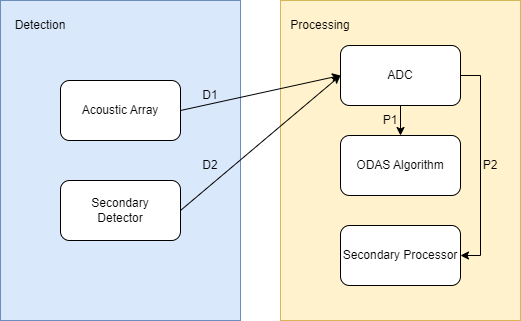
\includegraphics[width=0.60\textwidth]{images/adc_diagram.drawio}
 \caption{describes the relation of ADC along with other subsystems and layers}
\end{figure}

\subsubsection{Assumptions}
The data collected from analog sensors is understood by the ADC and is able to be converted, and the converted digital data is able to be interpreted and processed by the ODAS algorithm and the secondary processor. 

\subsubsection{Responsibilities}
The ADC subsystem is responsible for connecting the real world with the digital system of the product.  The detection layer wouldn't be able to produce any results without its data being processable, and the other subsystems in the processing layer wouldn't have any data to process. 

\subsubsection{Subsystem Interfaces}
\begin {table}[H]
\caption {Subsystem interfaces} 
\begin{center}
    \begin{tabular}{ | p{2cm} | p{6cm} | p{4cm} | p{4cm} |}
    \hline
    ID & Description & Inputs & Outputs \\ \hline
    \#D1/D2 & Analog Data Input & \pbox{3cm}{Acoustic Data \\ Secondary Detector Data} & \pbox{3cm}{Digitized Data}  \\ \hline
    \#P1 & Sending to ODAS & \pbox{3cm}{N/A} & \pbox{3cm}{Digitized Data}  \\ \hline
    \#P2 & Sending to Secondary Processor & \pbox{3cm}{N/A} & \pbox{3cm}{Digitized Data}  \\ \hline
    \end{tabular}
\end{center}
\end{table}

\subsection{ODAS Algorithm}
ODAS is an open source software developed for taking in multiple audio data sources and compiling it into usable data streams. For the purposes of the ARGOOSE system, ODAS will utilize a modified sourcing code to locate the sound of drones that are detected within the area of operation. At default, ODAS detects raw sounds and locations based off of the ReSpeaker array. This information is compiled and displayed on the software to pinpoint location and event data. Data streams will come in from the ADC on detected sound patterns, will be identified and manipulated by ODAS and then forwarded on to the Raspberry pi controller to display and interpret relevant data.

\begin{figure}[h!]
	\centering
 	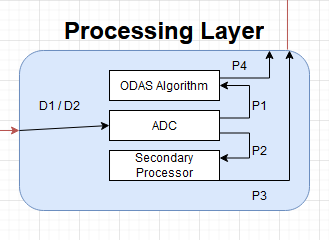
\includegraphics[width=0.50\textwidth]{images/processing}
 \caption{Example subsystem description diagram}
\end{figure}

\subsubsection{Assumptions}
ODAS algorithmic data processing will accurately detail drone detection and forward data streams that are relevant and interpretable by the Raspberry Pi.
Information received from the ADC will be in a format that is accurately analyzable by the ODAS algorithm.

\subsubsection{Responsibilities}
ODAS is responsible for generating the positional and occurrence data from the raw data stream of the ADC. It is the key component is generating the sample necessary for the controller to determine when and where drone detections should occur.

\subsubsection{Subsystem Interfaces}

\begin {table}[H]
\caption {Subsystem interfaces} 
\begin{center}
    \begin{tabular}{ | p{1cm} | p{6cm} | p{3cm} | p{3cm} |}
    \hline
    ID & Description & Inputs & Outputs \\ \hline
    \#RS01 & ODAS Algorithm & \pbox{3cm}{ADC Data Stream} & \pbox{3cm}{Compiled Detection Data to Controller}  \\ \hline
    \end{tabular}
\end{center}
\end{table}

\subsection{Secondary Processing Subsystem}
The secondary processing subsystem is responsible for activation of the secondary sensors and detection system after the object is suspected to be a drone.

\begin{figure}[h!]
	\centering
 	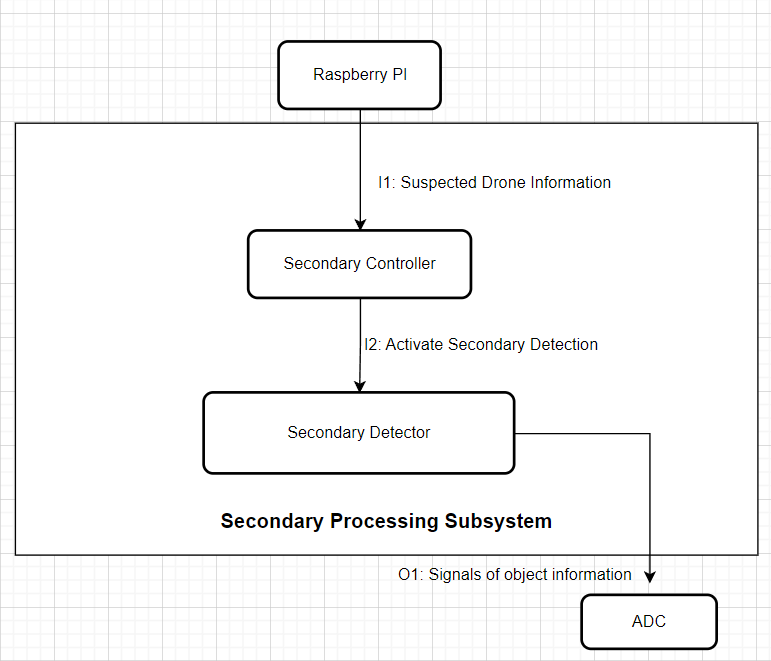
\includegraphics[width=0.60\textwidth]{images/Secondary Processing_Subsystem.png}
 \caption{Secondary Processing Subsystem}
\end{figure}

\subsubsection{Assumptions}
This subsystem assumes that it has an object that is potentially a drone and this information is given by the raspberry pi. 

\subsubsection{Responsibilities}
The primary responsibility of this subsystem is to confirm that the object is a drone. It activates the secondary detection sensors which sends the signals to ADC and these signals are sent through ODAS algorithm to the raspberry pi.

\subsubsection{Subsystem Interfaces}

\begin {table}[H]
\caption {Subsystem interfaces} 
\begin{center}
    \begin{tabular}{ | p{1cm} | p{6cm} | p{3cm} | p{3cm} |}
    \hline
    ID & Description & Inputs & Outputs \\ \hline
    \#I1 & Secondary Controller & \pbox{3cm}{Drone Information} & \pbox{3cm}{Signal to secondary detector}  \\ \hline
    \#I2 & Secondary detector & \pbox{3cm}{Activate secondary sensor} & \pbox{3cm}{N/A}  \\ \hline
    \end{tabular}
\end{center}
\end{table}